\chapter{热力学基础}
\section{选择题}
\exercise C

\solve 
等体加热内能增大,A错;

等温过程内能不变,$\Delta E = 0$,$Q+A>0$,$Q<0$,B错;

由$PV=nRT$,$V\uparrow$,则$T\uparrow$,则$\Delta E>0$,又$A<0$,则$Q>0$,C正确;

绝热压缩,$A>0$,$Q=0$,则$\delta E>0$,D错。

\exercise A

\solve 
由容积不变知为等体过程,则${Q_V} = \nu {C_V}({T_2} - {T_1})$,$H_2$为双原子分子,${C_V} = \frac{5}{2}R,$ \ce{NH3}为多原子分子,$C_V=3R$(本章未提及),则A正确。


\exercise B

\solve 由图中ab及cd围成面积知$\Delta {E_{ab}} = \Delta {E_{cd}}$,$A_{ab} < {A_{cd}}$,由$\Delta E = Q + A$知$Q_{ab} > {Q_{cd}}$,又${Q_{ab}}= 0$,所以${A_{cb}} < 0$,即$C < 0$,故选B。


\exercise D

\solve 等温:$\delta T=0$

等压:由$PV=nRT$,$\frac{V_2}{V_1}=\frac{T_2}{T_1}\Rightarrow \left|\delta T\right|=T_1$

绝热:由$TV^\gamma=C_2$知$(\frac{V_1}{V_2})^{\gamma-1}=\frac{T_2}{T_1}\Rightarrow \left|\delta T\right|=\left|[1-(\frac{1}{2})^{\gamma-1}]T_1\right|$

则选D。

\exercise D

\solve 绝热线与等温线只有一个交点,A错;

由$PV=nRT$,两者内能变化量相同,但做功不同,则吸热量不同,B错;

曲线下围成面积不同,C错;

由$PV=nRT$,D对。

\exercise D

\solve 等压过程,系统对外做功$A=\nu R(T_2-T_1)$,吸热$Q_P=\nu C_P(T_2-T_1)$,则$\frac{W}{Q}=\frac{A}{Q_P}=\frac{R}{C_P}=\frac{1}{1+\frac{5}{2}}=\frac{2}{7}$

故选D。

\exercise C

\solve $\eta=1-\frac{T_1}{T_2}$,易知BCC'和ADD'分别为等温线,则$\eta_1=\eta_2$;
由图,BCD下面积小于BCD',则$W_1<W_2$,故选C。

\exercise C

\solve 体积增大,则W>0;

$T_a=\frac{2p_1V_1}{nR}=T_b$,则$\Delta E=0$,故选C。

\exercise B

\solve A错,绝热斜率应该比等温线绝对值大;

B是合理的;

C、D选项,绝热线不能相交;

故选B。

\exercise D

\solve 假设可行,则$\eta=1000/1600=62.5\%$;

而由卡诺循环,$\eta=1-\frac{T_2}{T_1}=25\%$,故选D。

\section{计算题}
\exercise $\frac{1}{2}(\frac{C}{V_1^2}-\frac{C}{V_2^2})$或$\frac{1}{2}(P_1V_1-P_2V_2)$\qquad 减少\qquad 放热

\solve $W = \int_{{V_1}}^{{V_2}} {p\di{V} = } \int_{V_1}^{V_2}{\frac{C}{{{V^3}}}\di{V}=}- \frac{1}{2}(\frac{C}{{{V_2}^2}}-\frac{C}{{{V_1}^2}})=\frac{1}{2}(P_1V_1-P_2V_2)$

由$PV = nRT,P{V^3} = C$得$T=\frac{C}{nRV^2}$,V增加,T减少,则气体内能减少

$\Delta E = \nu {C_V}({T_2}-{T_1})= \frac{{{C_V}({p_2}{V_2} - {p_1}{V_1})}}{R} = \frac{C_V}{R}(\frac{C}{V_2^2}-\frac{C}{V_1^2})$

$\Delta Q = \Delta  + A = (\frac{C_V}{R} - \frac{1}{2})(\frac{C}{V_2^2} - \frac{C}{V_1^2}) < 0$

所以放热。

\exercise 不重合\qquad$\gamma$不同\qquad 不重合

\solve
$\gamma$不同,则其函数型$pV^\gamma=C$不同。

\exercise 500\qquad700

\solve 
等压过程中,$A=p\Delta V=\nu \Delta T$,单原子分子$C_{P1}=\frac{5}{2}R$

$Q_1=\nu C_{P1} \Delta T=\dfrac{5}{2}A=500\mathrm{J}$

$Q_2=\nu C_{P2} \Delta T=\dfrac{7}{2}A=700\mathrm{J}$

\exercise 温度\qquad 过程\qquad 做功\qquad 传递热量

\exercise 2/3\qquad$2S_1$

\solve
$\eta =1-\frac{T_0}{3T_0}=\frac{2}{3}$

$W=\frac{S_1}{1-\eta}-S_1=2S_1$

\exercise 1/3\qquad200J

\solve
$\eta =1-\frac{T_2}{T_1}=\frac{1}{3}$

$W=\frac{T_2}{T_1-T_2}=2\mathrm{J}$

$A=\frac{Q_2}{W}=200\mathrm{J}$

\exercise =\qquad >

\solve 两种气体对外做功即为abcda围成的面积,相等。

$\eta=\frac{W}{Q},W$相同,由$pV=nRT$知温度变化量也相同;

ab过程为等压过程,且$C_{\text{\RNum{1}}}<C_\text{\RNum{2}}$,则$Q_{\text{\RNum{1}}}<Q_{\text{\RNum{2}}}$,则有$\eta_{\text{\RNum{1}}}>\eta_{\text{\RNum{2}}}$

\exercise $\frac{1}{2}p_0V_0\qquad 9p_0V_0$

\solve W即为1\to2\to3\to1围成的面积,易得$W=\frac{1}{2}p_0V_0$

$\Delta E=\nu C_V\Delta T=\frac{3C_Vp_0V_0}{R}=\frac{15p_0V_0}{2}$

对外做功为1\to2下的面积,即$A=\frac{3p_0V_0}{2}$,则$Q=\Delta E+A=9p_0V_0$

\exercise 3R

\solve
%gxf对原解答做了改动
$A=\frac{3p_1V_1}{2}$,$\Delta T=\frac{\Delta(PV)}{\nu R}=\frac{3p_1V_1}{R}$

$\Delta E=\nu C_V\Delta T=\frac{15p_1V_1}{2}$

$Q=\Delta E+A=9p_1V_1$

\therefore$C=\frac{Q}{\Delta T}=3R$

\exercise 40J\qquad 120J

\solve 由EBCE循环系统对外做功70J,EDAE过程外界对系统做功30J,则一次循环过程系统对外做净功40J;

由于AEB为绝热过程,则$Q_{EAB}=0$,由$Q=\Delta E+A$知:

$W+\Delta E=Q_{BC}+Q_{CED}+Q_{DA}$

由于理想气体一次循环中的内能不变,则$\Delta=500$,则有$40=-30+Q_{CED}-50$,则
$Q_{CED}=120\mathrm{J}$

又因为CED为等体过程,则$A_{CED}=0,\Delta E=120\mathrm{J}$.

\section{解答题}

\exercise

\solve 由\[Q = \Delta E + A\]
知\[\eta=1-\frac{{\Delta {E_{BC}} + {A_{BC}}}}{{\Delta {E_{DA}} + A{  _{DA}}}}\]
\[{A_{BC}}=-\frac{1}{2}({p_B} + {p_C})({V_B} - {V_C})\]
\[\Delta {E_{BC}} = \nu {C_V}({T_C} - {T_B}) = \frac{{{C_V}({p_C}{V_C} - {p_B}{V_B})}}{R} = \frac{1}{{\gamma  - 1}}({p_C}{V_C} - {p_B}{V_B})\]
\[ \Rightarrow {Q_{BC}} = \frac{{\gamma  + 1}}{{2(\gamma  - 1)}}({p_C}{V_C} - {p_B}{V_B}) - \frac{1}{2}({p_C}{V_B} - {p_B}{V_C})\]
由于\[\frac{{{p_C}}}{{{V_C}}} = \frac{{{p_B}}}{{{V_B}}}\]
所以\[{p_C}{V_B} = {p_B}{V_C}\]
则\[{Q_{BC}} = \frac{{\gamma  + 1}}{{2(\gamma  - 1)}}({p_C}{V_C} - {p_B}{V_B})\]
同理\[{Q_{DA}} = \frac{{\gamma  + 1}}{{2(\gamma  - 1)}}({p_A}{V_A} - {p_D}{V_D})\]
则\[\eta  = 1 + \frac{{{Q_{BC}}}}{{{Q_{DA}}}} = 1 + \frac{{{T_C} - {T_B}}}{{{T_A} - {T_D}}}\]
在绝热过程AB中\[{T_B}{V_B}^{\gamma  - 1} = {T_A}{V_A}^{\gamma  - 1}\]
\[{p_B}^{\gamma  - 1}{T_B}^{ - \gamma } = {p_A}^{\gamma  - 1}{T_A}^{ - \gamma }\]
则有\[{T_B}^{\gamma+1}{\left(\frac{V_B}{p_B}\right)^{\gamma  - 1}} = {T_A}^{\gamma  + 1}{\left(\frac{V_A}{p_A}\right)^{\gamma  - 1}}\]
则\[\frac{{{T_B}}}{{{T_A}}} = \sqrt[{\gamma+1}]{{{{\left(\frac{V_A/p_A}{V_B/p_B}\right)}^{\gamma  - 1}}}} = \sqrt[{\gamma  + 1}]{{{{\left(\frac{V_D/p_D}{V_C/p_C}\right)}^{\gamma-1}}}} = \frac{{{T_D}}}{{{T_C}}}=k\]
则\[\eta  = 1 + \frac{T_C-T_B}{T_A-T_D} = 1 - \frac{T_B}{T_A}\]

\exercise

\solve

(1)
\begin{gather*}
A = \int_{{V_0}}^{6{V_0}} p\di{V}=7{p_0}{V_0}\\
\Delta E = \nu {C_V}({T_C} - {T_A}) = \frac{{5\nu R({T_C} - {T_A})}}{2} = \frac{5}{2}(6{p_0}{V_0} - 3{p_0}{V_0}) = \frac{{15}}{2}{p_0}{V_0}\\
Q = \Delta E + A = \frac{{29}}{2}{p_0}{V_0}
\end{gather*}

(2)
\[\di{S}=\frac{\di{Q}}{T}\footnote{该公式会在下一章介绍。}=\frac{{dE +p\di{V}}}{T}=\frac{{\nu{C_V}}}{T}\di{T}+\frac{{\nu R}}{V}\di{V}\]
则
\begin{align*}
\Delta S&= \int_{T_1}^{{T_2}}\frac{{\nu {C_V}}}{T}\di{T}+\int_{{V_1}}^{{V_2}} {\frac{{\nu R}}{V}\di{V}}\\
&=\frac{{5\nu R}}{2}\ln\frac{6{p_0}{V_0}/\nu R}{3{p_0}{V_0}/\nu R}+\nu R\ln \frac{{6{V_0}}}{{{V_0}}}\\
&= 29.29\mathrm{J/K}
\end{align*}

\exercise

\solve
(1)
%\begin{figure}[!h]
%	\centering
%	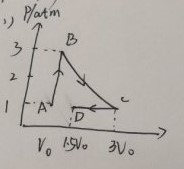
\includegraphics[width=0.35\textwidth]{Chp11_23.jpeg}
%\end{figure}
\tikzset{
	arrow1/.style = {
		draw = black, thick, -{Latex[length = 4mm, width = 1.5mm]},
	}
}
\begin{figure}[!h]
	\centering
	\begin{tikzpicture}[scale=1.2]
	%坐标轴和点
	\draw (0,0) node[below left] {$O$};
	\draw [->] (0,0) -- (4,0) node[right] {$V/V_0$};
	\draw [->] (0,0) -- (0,4) node[right] {$P/\mathrm{atm}$};
	\foreach \x in {1,1.5,3}
	{	
		\draw (\x,-0.05) -- (\x,0.05)
		node[below,outer sep=4pt,fill=white,font=\small]
		{\x} ({\x},0);
	}
	\foreach \y in {1,2,3}
	{	
		\draw (-0.05,\y) -- (0.05,\y)
		node[left,outer sep=3pt,fill=white,font=\small]
		at (0,{\y}) {{\y}};
	}
	\coordinate (A) at (1,1);
	\coordinate (B) at (1,3);
	\coordinate (C) at (3,1);
	\coordinate (D) at (1.5,1);
	\draw (A) node[below left] {$A$};
	\draw (B) node[above right] {$B$};
	\draw (C) node[below right] {$C$};	
	\draw (D) node[below right] {$D$};
	%线
	\draw [dashed,-] (0,1) -- (A);
	\draw [dashed,-] (1,0) -- (A);
	\draw [dashed,-] (0,3) -- (B);
	\draw [] (A) -- (1,2);
	\draw [-] (1,2) -- (B);
	\draw [->,domain=1:1.8,smooth] plot(\x,{3/\x});
	\draw [-,domain=1.8:3,smooth] plot(\x,{3/\x}) node at (2.5,1.8){$y=3/x$};
	\draw [->] (C) -- (2.25,1);
	\draw [-] (2.25,1) -- (D);
	\draw [dashed,-] (D) -- (1.5,0);
	\end{tikzpicture}
\end{figure}

(2)%gxf对原解答做了改动
\[\nu  = \frac{m}{M} = 0.1\mathrm{mol}\]
\[\frac{T_B}{T_A}=\frac{p_B}{V_B}{p_A}{V_A} = 3 \Rightarrow {T_B} = 3{T_A} = 900\mathrm{K}\]
同理,$\frac{T_D}{T_C}=0.5$,且有$T_C=T_B$,则:
\[\Delta E =\nu {C_V}({T_D}-{T_A})= 311\mathrm{J}\]
\[A =\nu R{T_B}\ln \frac{3{V_0}}{V_0}-\frac{{3P_0V_0}}{2}\]
由${p_0}{V_0} = nR{T_A}$得:
\[\frac{{3{p_0}{V_0}}}{2} = 374.13\mathrm{J}\]
则\[A = 450.65\mathrm{J}\]
\[Q = \Delta E+A = 762.42\mathrm{J}\]

\exercise

\solve 由下一章知识,\[{C_V} = \frac{i}{2}R,{C_p} = \frac{{i + 2}}{2}R\]
则
\[\gamma=\frac{{i + 2}}{i}\]
因为是绝热过程,则有
\[{T_0}{V_0}^{\gamma-1}={T_\text{\RNum{1}}}{(\frac{V_0}{2})^{\gamma-1}}= {T_\text{\RNum{2}}}{(\frac{{3{V_0}}}{2})^{\gamma-1}}\]
解得
\[{T_\text{\RNum{1}}} = {2^{\frac{2}{i}}}{T_0},{T_\text{\RNum{2}}} = {(\frac{2}{3})^{\frac{2}{i}}}{T_0}\]
则
\[A = \frac{{\nu R}}{{\gamma-1}}({(\frac{2}{3})^{\frac{2}{i}}}{T_0} - {T_0}) + \frac{{\nu R}}{{\gamma  - 1}}({2^{\frac{2}{i}}}{T_0}-{T_0}) = \frac{{i\nu R{T_0}}}{2}[{(\frac{2}{3})^{\frac{2}{i}}} + {2^{\frac{2}{i}}} - 2]\]